\documentclass[conference]{IEEEtran}
% Compile on Overleaf (pdfLaTeX + BibTeX). Uses only standard packages.
\usepackage{cite}
\usepackage{amsmath,amssymb}
\usepackage{graphicx}
\usepackage{booktabs}
\usepackage{algorithm}
\usepackage{algpseudocode}
\usepackage{url}
\graphicspath{{figures/}}

\begin{document}

\title{EarlyShield: An Explainable Behavioral Machine Learning Framework for Early Ransomware Detection and Secure Automated Recovery}

% NOTE: fill in department and e-mail addresses; confirm the guide's name
% spelling (the project README spells it "Neha Seirah Biju").
\author{
\IEEEauthorblockN{Chandana R, Venkat Mokshith K S, Susmitha B S}
\IEEEauthorblockA{[Department]\\
Presidency University, Bengaluru, India\\
\{[email1], [email2], [email3]\}}
\and
\IEEEauthorblockN{Neha Seirah Biju}
\IEEEauthorblockA{Assistant Professor, [Department]\\
Presidency University, Bengaluru, India\\
[email]}
}

\maketitle

\begin{abstract}
Most machine-learning ransomware detectors are evaluated by classification accuracy on held-out feature vectors, which says little about whether a running system stops an attack before data is lost. We present EarlyShield, an end-to-end framework that couples a behavioral Random Forest detector with per-alert SHAP explanations and an automated recovery engine built on an integrity-verified shadow-copy vault. On held-out data the detector reaches 96.79\% accuracy (F1 0.968, ROC-AUC 0.98). We then evaluate the deployed system live over 225 trials, in which a separate process runs four ransomware behaviors or nine benign workloads against a monitored folder. On a final 90-trial run over unseen corpora, EarlyShield detected 33 of 36 attacks with a median time to detection of 5.3\,s. It restored every file, leaving no artifacts, in all 27 burst, throttled and copy-then-delete trials, and raised no false alarm on 42 trials of seven ordinary workloads. After adding an incident follow-up step, a further 36 attack trials were all detected and fully recovered. Two weaknesses remain: slow in-place encryption scores 0.48--0.56, on the decision boundary, and gzip archiving still triggers a reversible response. The live evaluation also exposed five feature-extraction defects and a false positive that the offline metrics had concealed.
\end{abstract}

\begin{IEEEkeywords}
ransomware detection, explainable AI, SHAP, random forest, automated recovery, behavioral analysis, real-time evaluation
\end{IEEEkeywords}

\section{Introduction}
Ransomware causes harm in the seconds to minutes during which it encrypts user data. Defenses must therefore be judged not only on whether they recognise an attack, but on how much data is irrecoverably lost by the time they do. Existing literature identifies several open gaps~\cite{urooj2022survey,vehabovic2022strategies}:
(i)~detecting attacks \emph{early}, before significant encryption;
(ii)~detecting previously unseen variants from behaviour rather than signatures;
(iii)~explaining each decision to the analyst who must act on it;
(iv)~integrating detection with automated, trustworthy recovery;
(v)~keeping false positives low; and
(vi)~evaluating under real-time conditions.

This paper addresses all six with a single deployable system and makes the following contributions:
\begin{itemize}
\item A behavioral detector over 11 per-window file-system and process features, which explains every alert with TreeSHAP~\cite{lundberg2020treeshap} (Section~\ref{sec:design}).
\item A recovery engine that quarantines rather than deletes, restores from a SHA-256 content-addressed vault, guards against restoring already-encrypted versions, and keeps an auditable action log. Every response is reversible (Section~\ref{sec:recovery}).
\item A live-system evaluation methodology that measures time to detection, files encrypted before detection, files lost after recovery and false alarms (Section~\ref{sec:eval}).
\item Evidence that offline accuracy can hide defects in real-time feature extraction: five such defects were found only by the live evaluation (Section~\ref{sec:lessons}).
\end{itemize}

\section{Related Work}
\textbf{Behavioral detection.} UNVEIL~\cite{kharraz2016unveil} detects ransomware in an instrumented sandbox by observing access to user data. CryptoDrop~\cite{scaife2016cryptolock} uses file-transformation indicators, among them entropy change, file-type change and similarity loss, to halt a process after a small number of files. It reported a median loss of 10 files. Hirano and Kobayashi~\cite{hirano2019storage} trained Random Forest, SVM and k-NN classifiers on storage-access patterns captured by a hypervisor. Surveys~\cite{urooj2022survey,vehabovic2022strategies} note that most ML approaches report offline accuracy on recorded behaviour logs, and that evaluation under live conditions is rare.

\textbf{Recovery.} ShieldFS~\cite{continella2016shieldfs} combines adaptive detection models with copy-on-write in a Windows filesystem driver and rolls back a malicious process's changes. Redemption~\cite{kharraz2017redemption} buffers storage I/O transparently and restores data after flagging a process. Both achieve strong guarantees through kernel-level integration. EarlyShield instead targets a portable user-space design and makes its recovery decisions explainable and auditable.

\textbf{Explainability.} SHAP~\cite{lundberg2017shap} attributes a prediction to its input features using Shapley values; TreeSHAP~\cite{lundberg2020treeshap} computes them exactly and efficiently for tree ensembles such as Random Forests~\cite{breiman2001rf}. We use it to attach a feature-level justification to every alert.

\section{System Design}\label{sec:design}
Fig.~\ref{fig:arch} shows the architecture. A watcher buffers file events from a monitored directory, and an aggregator turns each observation window of length $W$ into a feature vector. A detector classifies the vector and explains the result. If the confidence reaches a threshold $\tau$, the recovery engine responds.

\begin{figure*}[t]
\centering
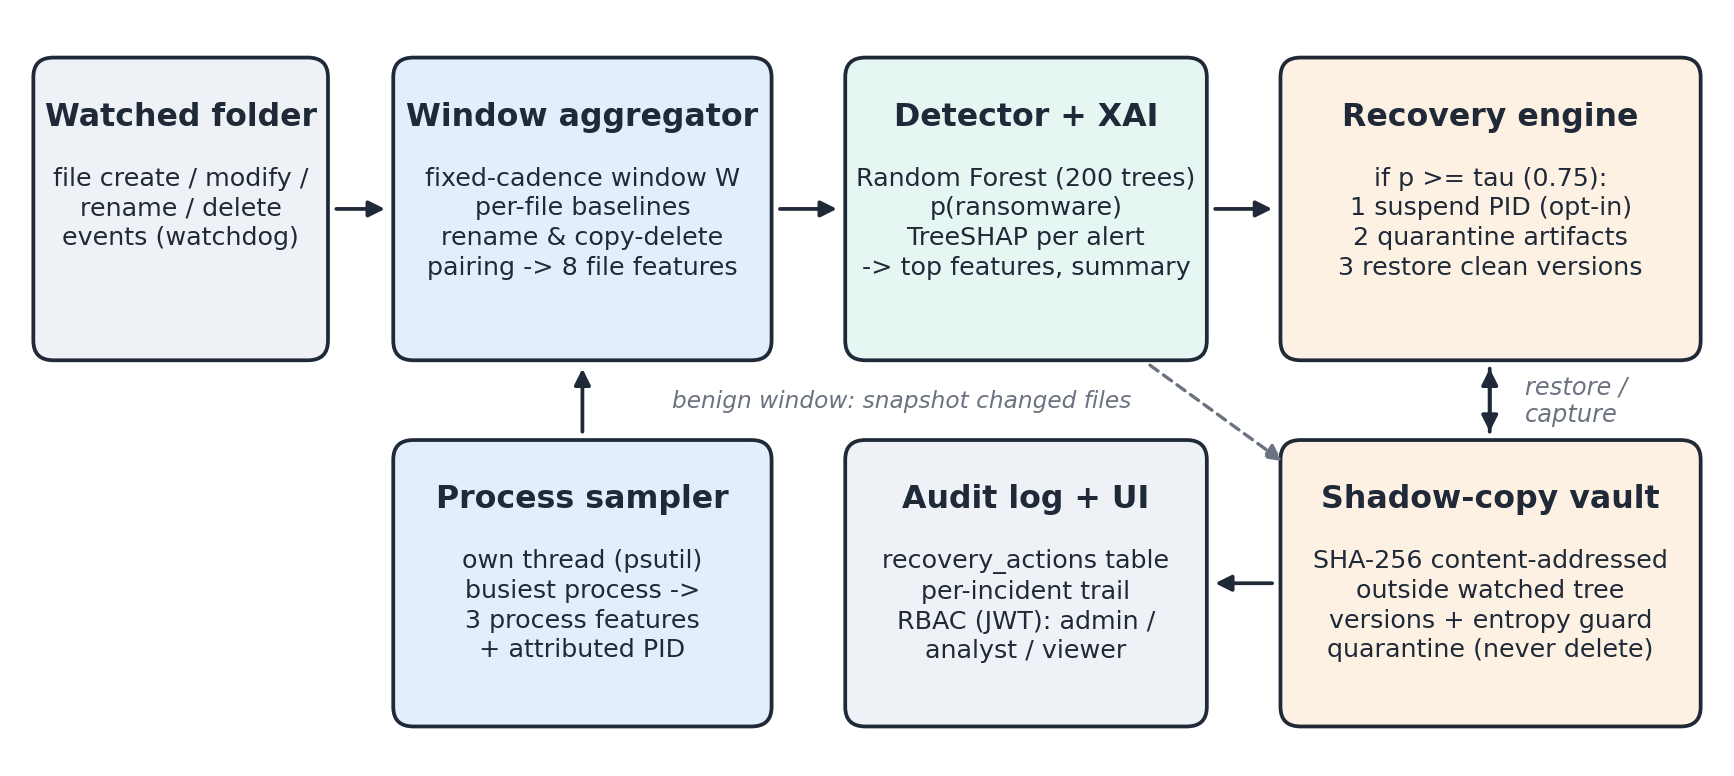
\includegraphics[width=0.82\textwidth]{architecture.png}
\caption{EarlyShield architecture. Windows run on a fixed cadence; process sampling runs on its own thread so that it never delays file analysis.}
\label{fig:arch}
\end{figure*}

\subsection{Behavioral Features}
Table~\ref{tab:features} lists the 11 features. Eight describe file activity; three describe the process that was most active during the window. Content is read at the \emph{end} of each window, from each file's final path after following rename chains (e.g.\ \texttt{a.txt}~$\rightarrow$~\texttt{a.txt.locked}), which avoids races with in-flight writes. Each file is compared with a \emph{baseline} recorded before the window: baselines are seeded for every file when monitoring starts and are carried across renames. When a new file \texttt{x.enc} appears while \texttt{x} is deleted in the same window, the two events are paired, so copy-then-delete encryption is judged against the original file's history. Entropy is \emph{content-aware}: a file that genuinely decompresses (gzip, bzip2, xz or an unencrypted zip member) is scored on its decompressed bytes. Legitimate archives therefore score like their contents, while ciphertext, ciphertext wrapped in a valid gzip stream, and password-protected archives still score close to 8 bits/byte.

\begin{table}[t]
\caption{Per-window behavioral features}
\label{tab:features}
\centering
\footnotesize
\begin{tabular}{@{}ll@{}}
\toprule
Feature & Definition \\
\midrule
file\_modification\_rate & files written (created or modified) per second \\
file\_rename\_rate & renames per second \\
file\_deletion\_rate & deletions per second \\
entropy\_mean & mean Shannon entropy of written content (bits/byte) \\
entropy\_delta & mean per-file change vs.\ pre-window baseline \\
extension\_change\_ratio & share of changed files whose extension changed \\
unique\_dirs\_touched & distinct directories affected \\
avg\_size\_change\_ratio & mean new size / previous size \\
process\_cpu\_percent & CPU share of most active process (0--100) \\
io\_write\_rate\_mb\_s & that process's write throughput \\
read\_write\_ratio & that process's bytes read / bytes written \\
\bottomrule
\end{tabular}
\end{table}

Precisely attributing a file write to the process that issued it requires kernel hooks (e.g.\ ETW or fanotify). Our user-space design approximates the responsible process as the one with the highest combined CPU and write activity in the window. Section~\ref{sec:eval} measures how well this works.

\subsection{Detector and Explanations}
Training on live ransomware requires an isolated malware laboratory, which was outside the scope of this work. We therefore train on 12{,}000 synthetic windows (6{,}000 per class) whose feature distributions follow behaviour reported in the literature~\cite{hirano2019storage,urooj2022survey,vehabovic2022strategies}. To keep the classes from being trivially separable, each class has two overlapping sub-populations. Benign windows are 80\% normal activity and 20\% ``bursty'' software such as backup and build tools. Ransomware windows are 75\% typical and 25\% ``stealthy'' low-and-slow attacks. We add 8\% Gaussian feature noise and flip 2\% of labels. The detector is a Random Forest~\cite{breiman2001rf} (200 trees, depth $\le 12$, $\ge 5$ samples per leaf). For every alert, TreeSHAP~\cite{lundberg2020treeshap} produces per-feature contributions, and these are rendered as a ranked chart and a one-sentence summary (e.g.\ ``flagged primarily due to a large fraction of files changing extension and high content entropy'').

\subsection{Secure Automated Recovery}\label{sec:recovery}
\textbf{Shadow-copy vault.} When monitoring starts, every file is snapshotted; after each benign window, the files that changed are snapshotted again (up to five versions per file). Blobs are stored under their own SHA-256 digest and written read-only, and the digest is re-checked before every restore, so a tampered backup is refused. Monitoring will not start if the vault lies inside the watched tree.

\textbf{Clean-version selection.} Slow attacks can encrypt a few files in windows that are scored benign, and those encrypted versions would then be snapshotted. When restoring, the engine therefore skips any version whose entropy exceeds the file's first-ever snapshot by more than $\delta = 1.5$ bits/byte, and it takes no snapshots while an incident is active.

\textbf{Response.} Algorithm~\ref{alg:response} runs when a window is flagged with confidence $p \ge \tau$. We set $\tau = 0.50$ from a calibration run (Section~\ref{sec:lessons}). The window before the detection is included, because an attack's first seconds often score as benign. Every action is reversible: files are moved to a quarantine inside the vault rather than deleted, and processes are suspended, not killed. Process suspension is opt-in. It refuses EarlyShield's own process tree, PIDs 0, 1 and 4, a protected-name list, any PID whose name changed since sampling (PID reuse), and any process that wrote nothing in the window. Every step is written, with its incident ID and actor, to an append-only audit table. \textbf{Incident follow-up.} An incident stays open for three windows after its last flagged one. During that time, windows scored below $\tau$ are still checked for files the vault has never seen (ransom notes, encrypted copies) and for files whose entropy has jumped by more than $\delta$. Matches are handled as in Algorithm~\ref{alg:response}, and each match extends the incident. Outside an incident the check does nothing, so it cannot cause false alarms. Access is governed by role-based control: viewers can only observe, analysts can restore and resume, and only administrators can change response settings.

\begin{algorithm}[t]
\caption{Automated response to a flagged window}
\label{alg:response}
\small
\begin{algorithmic}[1]
\Require changes $C$ of this and the previous window; confidence $p$; attributed PID $q$
\If{$p < \tau$} \Return alert only \EndIf
\State open or continue incident $I$; cutoff $t_c \gets$ incident start $- W/2$
\If{auto-suspend \textbf{and} $q$ passes all safety checks} \State suspend $q$ \EndIf
\For{each original path $f$ in $C$}
  \State $v \gets$ newest version of $f$ captured before $t_c$ with entropy $\le H_0(f)+\delta$
  \If{$v = \varnothing$ \textbf{and} $f$ is new in this window} quarantine $f$ \Comment{e.g.\ ransom note}
  \ElsIf{$v \neq \varnothing$}
    \State quarantine renamed/modified copies of $f$
    \State verify SHA-256 of $v$; atomically restore $f \gets v$
  \EndIf
\EndFor
\State log every action under $I$
\end{algorithmic}
\end{algorithm}

\subsection{Implementation}
The backend is written in Python with FastAPI (Watchdog for file events, psutil for process sampling, scikit-learn and SHAP for detection, PostgreSQL for users and the audit log). The frontend is a React dashboard that shows the threat gauge, the SHAP chart, the detection timeline and the recovery log. Everything is packaged with Docker Compose. Because inotify events do not cross Docker Desktop bind mounts reliably, the watcher uses a 1\,s polling observer.

\section{Evaluation}\label{sec:eval}
\subsection{Offline Classification}
On a stratified 80/20 split (9{,}600/2{,}400 windows) the detector achieves the results in Table~\ref{tab:offline}. The confusion matrix has 39 false positives and 38 false negatives out of 1{,}200 windows per class. These figures describe separability of the \emph{synthetic} distributions only; the rest of this section measures the deployed system.

\begin{table}[t]
\caption{Offline classification (held-out synthetic windows)}
\label{tab:offline}
\centering
\footnotesize
\begin{tabular}{@{}cccccc@{}}
\toprule
Accuracy & Precision & Recall & F1 & ROC-AUC & 5-fold CV F1 \\
\midrule
0.9679 & 0.9675 & 0.9683 & 0.9679 & 0.980 & 0.9711 $\pm$ 0.0029 \\
\bottomrule
\end{tabular}
\end{table}

\subsection{Live-System Methodology}
Each trial builds a fresh corpus of 100 office-style files (text, CSV and JSON, 2--40\,KB, five folders) and starts the real monitor, detector and recovery engine with an empty vault. After one quiet window plus a random offset, so that attacks begin at a random point inside a window, a \emph{separate process} runs one workload. That process logs a timestamp for every file it touches, which lets us count exactly how many files were encrypted before detection. Afterwards we hash every corpus file against its original.

The four ransomware behaviours are: \emph{burst}, which overwrites every file with random bytes and renames it to \texttt{.locked} as fast as possible; \emph{throttled}, the same at 10 files/s; \emph{slow\_inplace}, which encrypts 2 files/s in place with no rename; and \emph{copy\_delete}, which writes \texttt{x.enc} and deletes \texttt{x}. All four drop a ransom note. Random bytes have the same byte statistics as cipher output. Seven ordinary benign workloads are document editing, a bulk rename of 100 files, creating a zip archive, copying the folder, converting \texttt{.txt} notes to \texttt{.md} (a legitimate mass change of extensions), a software install (60 new high-entropy binaries) and a photo import. Two harder cases are \emph{gzip\_compress}, which archives files to \texttt{x.csv.gz} and deletes the originals, the same shape as copy-then-delete, and \emph{legit\_encrypt}, a user encrypting their own files, which is behaviourally identical to ransomware and is expected to alarm. Attacks ran at $W \in \{2, 5, 10\}$\,s with three trials each. Slow attacks were stopped after 40\,s. We report four runs: a first run (51 trials, $\tau = 0.75$, five benign workloads), a calibration run (54 benign trials) a final run (90 trials, all workloads, $\tau = 0.50$) on corpora generated from seeds not used before, and a follow-up run (36 attack trials, new seeds) after incident follow-up was added. Detection time is taken when analysis of the flagged window finished, so it excludes the time spent recovering. All trials ran on one Windows 11 desktop with ordinary applications open. Auto-suspend was disabled; we measure attribution instead.

\subsection{Results}
Table~\ref{tab:live} summarises the final run; the first run is reported where it differs.

\begin{table}[t]
\caption{Final live-system run ($\tau = 0.50$, unseen corpora)}
\label{tab:live}
\centering
\footnotesize
\setlength{\tabcolsep}{3.2pt}
\begin{tabular}{@{}lccccc@{}}
\toprule
Workload & Trials & Detected & Max $p$ & Median TTD & Files lost \\
\midrule
burst & 9 & 9 & 0.92--0.94 & 4.8\,s & 0 \\
throttled & 9 & 9 & 0.79--0.95 & 4.1\,s & 0 \\
copy\_delete & 9 & 9 & 0.85--0.95 & 7.6\,s & 0 \\
slow\_inplace & 9 & 6 & 0.48--0.55 & 7.9\,s & 0--80 \\
\midrule
7 ordinary benign & 42 & 0 & $\le 0.23$ & -- & -- \\
gzip\_compress & 6 & 6 & 0.57--0.62 & -- & -- \\
legit\_encrypt & 6 & 6 & 0.87--0.90 & -- & -- \\
\bottomrule
\end{tabular}
\end{table}

\textbf{Detection and false positives.} The final run detected 33 of 36 attacks, with a median time to detection (TTD) of 5.3\,s, a 90th percentile of 9.1\,s and a maximum of 17.6\,s. No trial of the seven ordinary benign workloads raised an alarm; the highest ransomware probability on any of their windows was 0.23. User-initiated encryption alarmed in every trial, as any behavioural detector must. The first run (five benign workloads, $\tau = 0.75$) detected all 36 attacks, including all nine \emph{slow\_inplace} trials, which shows how close that attack sits to the boundary.

\textbf{Early detection (gap i).} Fig.~\ref{fig:damage} contrasts the damage done before detection with the data lost after recovery (first run). Burst encrypts all 100 files in about 0.2\,s, faster than any window-based detector can react, yet every file was recovered in all 27 burst, throttled and copy-then-delete trials of the final run. For the throttled attack in the first run, the number of files encrypted before detection grew with the window: 27, 41 and 73 at $W = 2$, 5 and 10\,s. $W$ is therefore the main lever for early detection.

\begin{figure}[t]
\centering
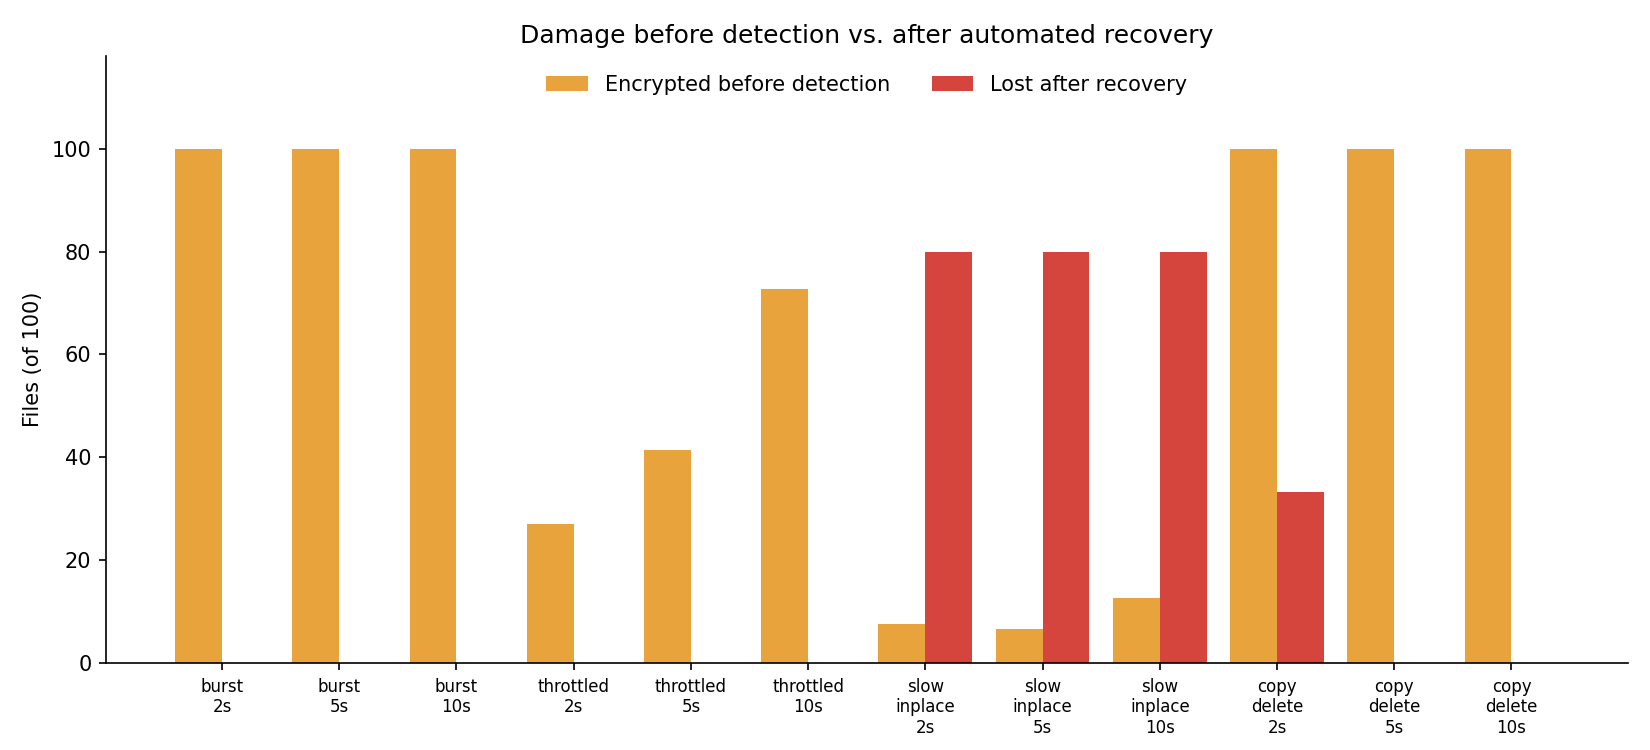
\includegraphics[width=\columnwidth]{damage_by_attack.png}
\caption{Mean files encrypted before detection vs.\ files lost after automated recovery (of 100), by attack and window size.}
\label{fig:damage}
\end{figure}

\textbf{Recovery (gap iv).} The response fired in all 33 detected trials and took 1.5\,s on average (at most 4.2\,s), including verifying the hash of each restored file. For burst, throttled and copy-then-delete, \emph{zero} files were lost and no \texttt{.locked}, \texttt{.enc} or ransom-note files remained. Slow in-place encryption is the exception. Its windows score 0.48--0.55, so an attack may cross $\tau$ in some windows and not in others. Files encrypted during windows below $\tau$ were not restored, which cost 11 and 79 files in two responded trials and 80 in each of the three undetected ones. In four responded trials nothing was lost. We then added incident follow-up (Section~\ref{sec:recovery}) and ran 36 further attack trials on new corpora. All 36 were detected (slow in-place at 0.52--0.56) with zero files lost and no artifacts left. The follow-up closes losses \emph{after} a detection, but it cannot help an attack none of whose windows reach $\tau$.

\textbf{Attribution.} The attributed process was never the attacker; the monitor typically blamed a web browser or another desktop application instead. A short-lived attacker can exit before the next process sample, and slow attackers write far less data than ordinary desktop applications do. Inside the container, where few processes are visible, a single throttled demonstration run suspended the correct attacker PID. Because attribution is unreliable on a busy desktop, auto-suspend is disabled by default. File recovery does not depend on attribution.

\subsection{Lessons from the Live Evaluation}\label{sec:lessons}
The first live run (one trial per attack, $W = 5$\,s) detected only burst and throttled. Inspecting the features of each window, together with the first end-to-end tests on a multi-core Windows host, revealed five defects in feature extraction rather than in the model:
(1)~baselines were recorded the first time a file \emph{changed}, i.e.\ after it had been encrypted, so \texttt{entropy\_delta} was always 0 and \texttt{avg\_size\_change\_ratio} always 1.0 for attacked files;
(2)~created files were not counted as file activity, so copy-then-delete produced a modification rate of 0;
(3)~\texttt{read\_write\_ratio} was computed against an already-overwritten counter and was always 0;
(4)~windows waited a full $W$ \emph{after} processing, and a full process scan takes 3--5\,s on Windows, so a ``5\,s'' window lasted about 10\,s;
(5)~per-process CPU exceeded 100\% on multi-core hosts and was rejected by input validation, which silently dropped every window.
After fixing these defects, without retraining or tuning the model, detection rose to 36/36 trials. None of the defects affected the 96.79\% offline accuracy, which is precisely why they went unnoticed.

The calibration run then added harder benign workloads and exposed a false positive: \emph{gzip\_compress} scored 0.78--0.91. Every threshold from 0.50 to 0.75 misfired on the same six gzip trials, and only 0.50 let recovery reach \emph{slow\_inplace}, so we set $\tau = 0.50$. Content-aware entropy (Section~\ref{sec:design}) was introduced in response and lowered gzip to 0.57--0.62. Because this fix was designed after seeing the calibration data, the final run used corpora from new seeds.

\section{Discussion and Limitations}
\textbf{Threshold trade-off.} With this model no single $\tau$ separates slow in-place encryption (0.48--0.55) from gzip archiving (0.57--0.62): at 0.65 gzip stops misfiring but slow in-place is never recovered; at 0.50 the reverse. We default to 0.50 because a wrong response is reversible (archives wait in quarantine) while a missed one loses data, and expose $\tau$ to administrators. Because the vault keeps pre-attack versions even when no response fires, an analyst can still restore files manually after an alert. A stronger fix is a data-preservation check: a compressed file whose content matches the deleted original is a transformation, not destruction.

\textbf{Training-data coverage.} The stealthy class assumes that most encrypted files also change extension, so in-place encryption lies outside the training distribution. We chose not to adjust the synthetic data to fit this benchmark, since that would overfit to the test. Training on recorded behaviour from real samples in a sandbox is the principled fix.

\textbf{Threats to validity.} The attacks are simulators. They do not reproduce process injection or memory-mapped I/O, nor intermittent encryption, which encrypts only alternating blocks so that files stay statistically close to the original and evade entropy-based detectors~\cite{sophos2021lockfile}. The results come from one machine and a 100-file corpus. Polling adds up to 1\,s of delay to event delivery.

\textbf{Vault security.} An attacker running as the same OS user could delete the vault. Production deployments need storage the attacker cannot reach, such as a privileged service, immutable object storage or a separate backup host.

\section{Conclusion}
EarlyShield shows that a portable, explainable detector coupled with integrity-verified, reversible recovery can undo fast and copy-then-delete ransomware completely: zero files lost in all 27 such live trials, with no false alarm on seven ordinary workloads. The live evaluation also showed that offline accuracy is a poor proxy for real-time effectiveness: it hid five feature-extraction defects and a false positive on gzip archiving. Incident follow-up then removed the remaining post-detection losses: 36 of 36 further attacks were recovered without loss. The remaining weakness is slow in-place encryption, which sits on the decision boundary, so a run whose windows all score below $\tau$ is missed. Future work includes training on sandboxed real-ransomware traces, a data-preservation check for archiving, kernel-assisted process attribution, and tamper-proof vault storage.

\bibliographystyle{IEEEtran}
\bibliography{references}

\end{document}
